\documentclass[11pt,a4paper,twoside]{report}
\usepackage[utf8]{inputenc}
\usepackage[T1]{fontenc}
\usepackage{lmodern}
\usepackage{amsmath}
\usepackage{amsfonts}
\usepackage{amssymb}
\usepackage{graphicx}
\usepackage{hyperref}
\usepackage{listings}
\usepackage{xcolor}
\usepackage{tikz}
\usepackage{float}
\usepackage{caption}
\usepackage{subcaption}
\usepackage{booktabs}
\usepackage{multirow}
\usepackage{array}
\usepackage{longtable}
\usepackage{enumitem}

% Definizione dei colori
\definecolor{codegreen}{rgb}{0,0.6,0}
\definecolor{codegray}{rgb}{0.5,0.5,0.5}
\definecolor{codepurple}{rgb}{0.58,0,0.82}
\definecolor{backcolour}{rgb}{0.95,0.95,0.92}

% Stile di codice
\lstdefinestyle{mystyle}{
    backgroundcolor=\color{backcolour},   
    commentstyle=\color{codegreen},
    keywordstyle=\color{magenta},
    numberstyle=\tiny\color{codegray},
    stringstyle=\color{codepurple},
    basicstyle=\ttfamily\footnotesize,
    breakatwhitespace=false,         
    breaklines=true,                 
    captionpos=t,                    
    keepspaces=true,                 
    numbers=left,                    
    numbersep=5pt,                  
    showspaces=false,                
    showstringspaces=false,
    showtabs=false,                  
    tabsize=2
}

\lstset{style=mystyle}

\usetikzlibrary{shapes,arrows,positioning,fit,backgrounds}

\title{\Huge{\textbf{EasyQuery}}\\\Large{Un Sistema Scalabile per la Gestione e l'Interrogazione dei Dati con Architettura Medallion}}
\author{Luca Borrelli \& Davide Mariani\\Università degli Studi dell'Aquila}
\date{\today}

\begin{document}

\maketitle
\tableofcontents

\chapter{Introduzione}

\section{Panoramica del Sistema}
EasyQuery è un sistema avanzato di gestione e interrogazione dei dati, progettato per semplificare l'interazione con grandi volumi di dati eterogenei. Implementa l'architettura Medallion (nota anche come architettura multi-hop o Delta) tipica delle moderne data lakehouse, strutturando i dati in layer progressivi (Bronze, Silver e Gold) che garantiscono scalabilità, affidabilità e prestazioni elevate.

Il sistema si distingue per:
\begin{itemize}
    \item Interfaccia conversazionale basata su AI per interrogazioni in linguaggio naturale
    \item Pipeline di trasformazione automatizzate tra i layer Bronze, Silver e Gold
    \item Gestione integrata della qualità e del lineage dei dati
    \item Scalabilità sia in termini di volume che di varietà dei dati
    \item Integrazione nativa con Google Cloud Platform (BigQuery, Cloud Storage, Dataplex)
\end{itemize}

\section{Obiettivi del Sistema}
EasyQuery si propone di risolvere diverse problematiche tipiche della gestione dei dati su larga scala:
\begin{itemize}
    \item Ridurre la complessità nell'accesso ai dati strutturati e non strutturati
    \item Eliminare la necessità di conoscenza approfondita di SQL per l'interrogazione dei dati
    \item Automatizzare la trasformazione e la pulizia dei dati
    \item Garantire la tracciabilità delle trasformazioni (data lineage)
    \item Ottimizzare le prestazioni per query analitiche complesse
    \item Scalare orizzontalmente per gestire volumi crescenti di dati
\end{itemize}

\chapter{Architettura del Sistema}

\section{Architettura Medallion}
EasyQuery implementa l'architettura Medallion, suddividendo i dati in tre layer principali:

\begin{figure}[H]
\centering
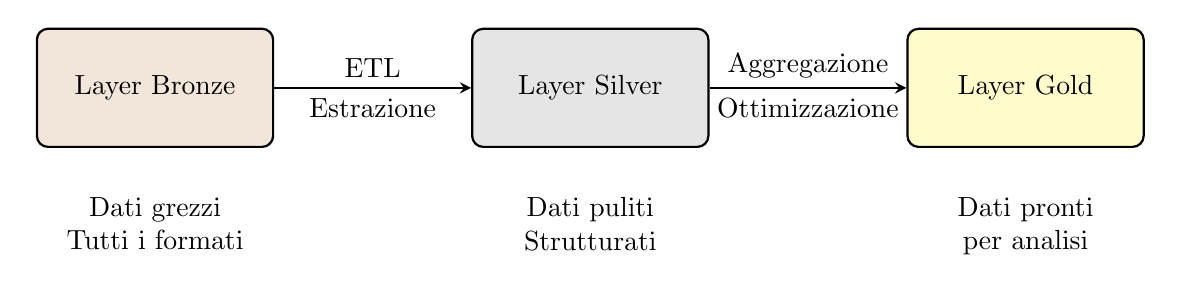
\begin{tikzpicture}[node distance=2.5cm, auto, thick]
    % Stili dei nodi
    \tikzstyle{layer}=[rectangle, rounded corners, minimum width=3cm, minimum height=1.5cm, text centered, draw=black, fill=blue!10]
    \tikzstyle{arrow}=[->, >=stealth, thick]
    
    % Nodi
    \node (bronze) [layer, fill=brown!20] {Layer Bronze};
    \node (silver) [layer, fill=gray!20, right=of bronze] {Layer Silver};
    \node (gold) [layer, fill=yellow!20, right=of silver] {Layer Gold};
    
    % Collegamenti
    \draw [arrow] (bronze) -- node[midway, above] {ETL} node[midway, below] {Estrazione} (silver);
    \draw [arrow] (silver) -- node[midway, above] {Aggregazione} node[midway, below] {Ottimizzazione} (gold);
    
    % Annotazioni
    \node[below=0.5cm of bronze, align=center, text width=3cm] {Dati grezzi\\Tutti i formati};
    \node[below=0.5cm of silver, align=center, text width=3cm] {Dati puliti\\Strutturati};
    \node[below=0.5cm of gold, align=center, text width=3cm] {Dati pronti\\per analisi};
\end{tikzpicture}
\caption{Architettura Medallion di EasyQuery}
\label{fig:medallion_architecture}
\end{figure}

\subsection{Layer Bronze}
Il layer Bronze rappresenta il punto di ingresso di tutti i dati nel sistema. Caratteristiche principali:
\begin{itemize}
    \item Conserva i dati grezzi nel loro formato originale
    \item Supporta un'ampia varietà di formati (CSV, JSON, PDF, immagini, ecc.)
    \item Arricchisce i dati con metadati di ingestion (timestamp, origine, tipo)
    \item Implementato utilizzando Google Cloud Storage per massima scalabilità
    \item Tutti i file sono tracciati in una tabella di metadati BigQuery
\end{itemize}

I metadati vengono registrati nella tabella \texttt{metadata\_store.bronze\_file\_metadata}, che include:
\begin{itemize}
    \item Percorsi GCS dei file originali
    \item Timestamp di caricamento
    \item Informazioni sul formato e sulla dimensione
    \item Stato di elaborazione
    \item Collegamenti ai dati nel layer Silver
\end{itemize}

\subsection{Layer Silver}
Il layer Silver contiene dati puliti, trasformati e strutturati:
\begin{itemize}
    \item Conversione di tutti i dati in formato Parquet per efficienza
    \item Normalizzazione dei nomi delle colonne (snake\_case)
    \item Inferenza e standardizzazione dei tipi di dati
    \item Estrazione di testo da documenti PDF e immagini tramite OCR
    \item Organizzazione in una struttura gerarchica basata su dominio e tipo
    \item Registrazione dei metadati e del lineage completo
\end{itemize}

I file Parquet vengono organizzati secondo una logica di dominio e contesto:
\begin{verbatim}
silver-layer-bucket/files/fin_str/csv/sales/monthly_report.parquet
\end{verbatim}

Dove:
\begin{itemize}
    \item \texttt{fin\_str}: Dominio finanziario, dati strutturati
    \item \texttt{csv}: Tipo di contenuto originale
    \item \texttt{sales}: Contesto applicativo
    \item \texttt{monthly\_report}: Nome del dataset
\end{itemize}

\subsection{Layer Gold}
Il layer Gold contiene dati ottimizzati per l'analisi:
\begin{itemize}
    \item Tabelle pre-aggregate pronte per query specifiche
    \item Ottimizzazione delle strutture dati per performance di interrogazione
    \item Materializzazione delle viste più utilizzate
    \item Implementato come tabelle BigQuery
    \item Metadati completi su origine e trasformazioni applicate
\end{itemize}

\section{Componenti del Sistema}
EasyQuery è composto da diverse componenti integrate:

\begin{figure}[H]
\centering
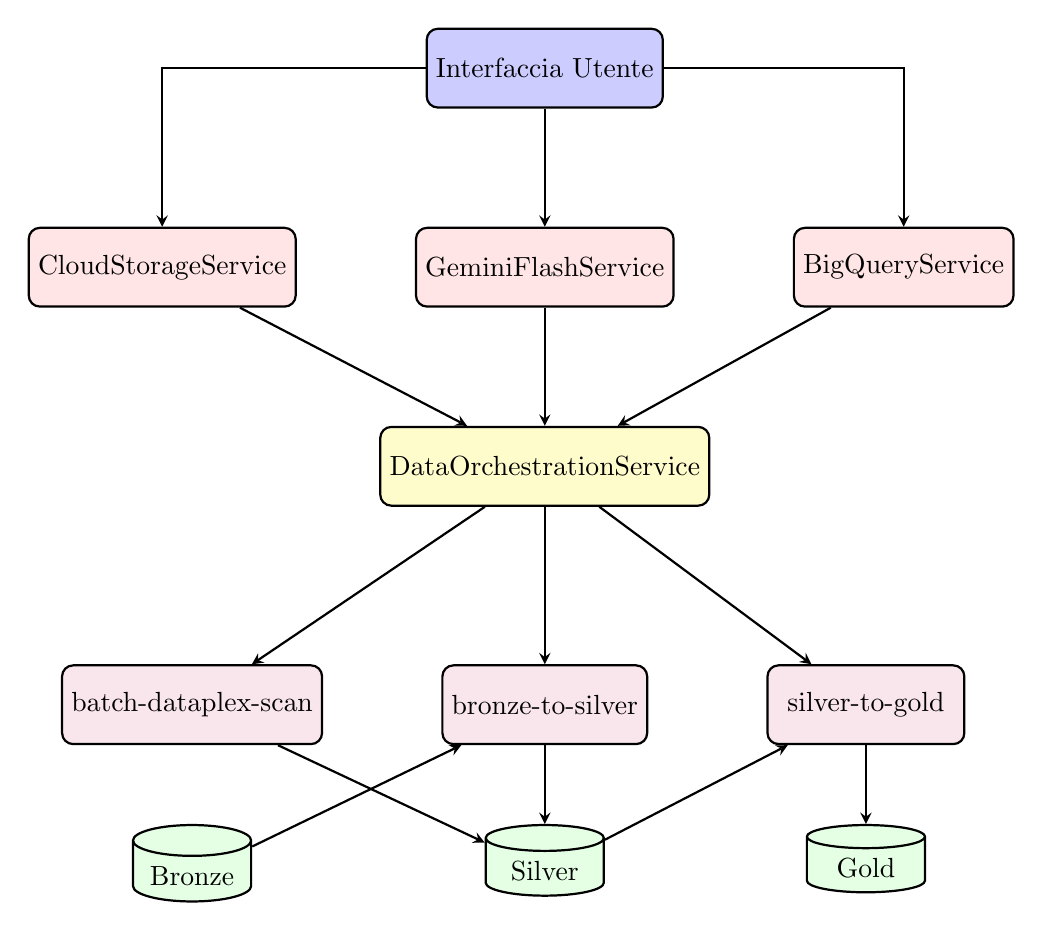
\begin{tikzpicture}[node distance=1.5cm, auto, thick]
    % Stili
    \tikzstyle{component}=[rectangle, rounded corners, minimum width=2.5cm, minimum height=1cm, text centered, draw=black, fill=blue!10]
    \tikzstyle{data}=[cylinder, draw=black, shape border rotate=90, aspect=0.3, fill=green!10, minimum height=0.8cm, minimum width=1.5cm]
    \tikzstyle{arrow}=[->, >=stealth, thick]
    
    % Frontend
    \node (ui) [component, fill=blue!20] {Interfaccia Utente};
    
    % Servizi principali
    \node (gemini) [component, fill=red!10, below=of ui] {GeminiFlashService};
    \node (bq) [component, fill=red!10, right=of gemini] {BigQueryService};
    \node (cs) [component, fill=red!10, left=of gemini] {CloudStorageService};
    \node (orch) [component, fill=yellow!20, below=of gemini] {DataOrchestrationService};
    
    % Cloud Functions
    \node (b2s) [component, fill=purple!10, below=2cm of orch] {bronze-to-silver};
    \node (s2g) [component, fill=purple!10, right=of b2s] {silver-to-gold};
    \node (dataplex) [component, fill=purple!10, left=of b2s] {batch-dataplex-scan};
    
    % Storage
    \node (bronze) [data, below=1cm of dataplex] {Bronze};
    \node (silver) [data, below=1cm of b2s] {Silver};
    \node (gold) [data, below=1cm of s2g] {Gold};
    
    % Collegamenti
    \draw [arrow] (ui) -- (gemini);
    \draw [arrow] (ui) -| (cs);
    \draw [arrow] (ui) -| (bq);
    \draw [arrow] (gemini) -- (orch);
    \draw [arrow] (bq) -- (orch);
    \draw [arrow] (cs) -- (orch);
    \draw [arrow] (orch) -- (b2s);
    \draw [arrow] (orch) -- (s2g);
    \draw [arrow] (orch) -- (dataplex);
    \draw [arrow] (bronze) -- (b2s);
    \draw [arrow] (b2s) -- (silver);
    \draw [arrow] (silver) -- (s2g);
    \draw [arrow] (s2g) -- (gold);
    \draw [arrow] (dataplex) -- (silver);
    
\end{tikzpicture}
\caption{Architettura delle componenti di EasyQuery}
\label{fig:components}
\end{figure}

\subsection{Frontend}
Implementato in Flutter, offre:
\begin{itemize}
    \item Interfaccia utente responsive e multi-piattaforma
    \item Box di ricerca per query in linguaggio naturale
    \item Funzionalità di caricamento intelligente dei file
    \item Visualizzazione avanzata dei risultati con grafici interattivi
    \item Modalità di esportazione e condivisione dei risultati
\end{itemize}

\subsection{Servizi Core}
\begin{itemize}
    \item \textbf{GeminiFlashService}: Integrazione con Google Gemini per elaborazione del linguaggio naturale e generazione di SQL
    \item \textbf{BigQueryService}: Gestione delle connessioni e delle query verso BigQuery
    \item \textbf{CloudStorageService}: Interazione con Google Cloud Storage per la gestione dei file
    \item \textbf{DataOrchestrationService}: Orchestrazione delle pipeline di elaborazione dati
\end{itemize}

\subsection{Cloud Functions}
\begin{itemize}
    \item \textbf{bronze-to-silver}: Trasforma i dati dal formato grezzo a Parquet strutturato
    \item \textbf{silver-to-gold}: Materializza tabelle ottimizzate per analisi
    \item \textbf{batch-dataplex-scan}: Aggiorna i metadati e mantiene aggiornata la Discovery di Dataplex
\end{itemize}

\chapter{Pipeline di Elaborazione Dati}

\section{Pipeline Bronze-to-Silver}

La pipeline Bronze-to-Silver rappresenta uno dei processi core di EasyQuery, responsabile della trasformazione dei dati grezzi in formati strutturati e ottimizzati.

\subsection{Processo di Trasformazione}

\begin{figure}[H]
\centering
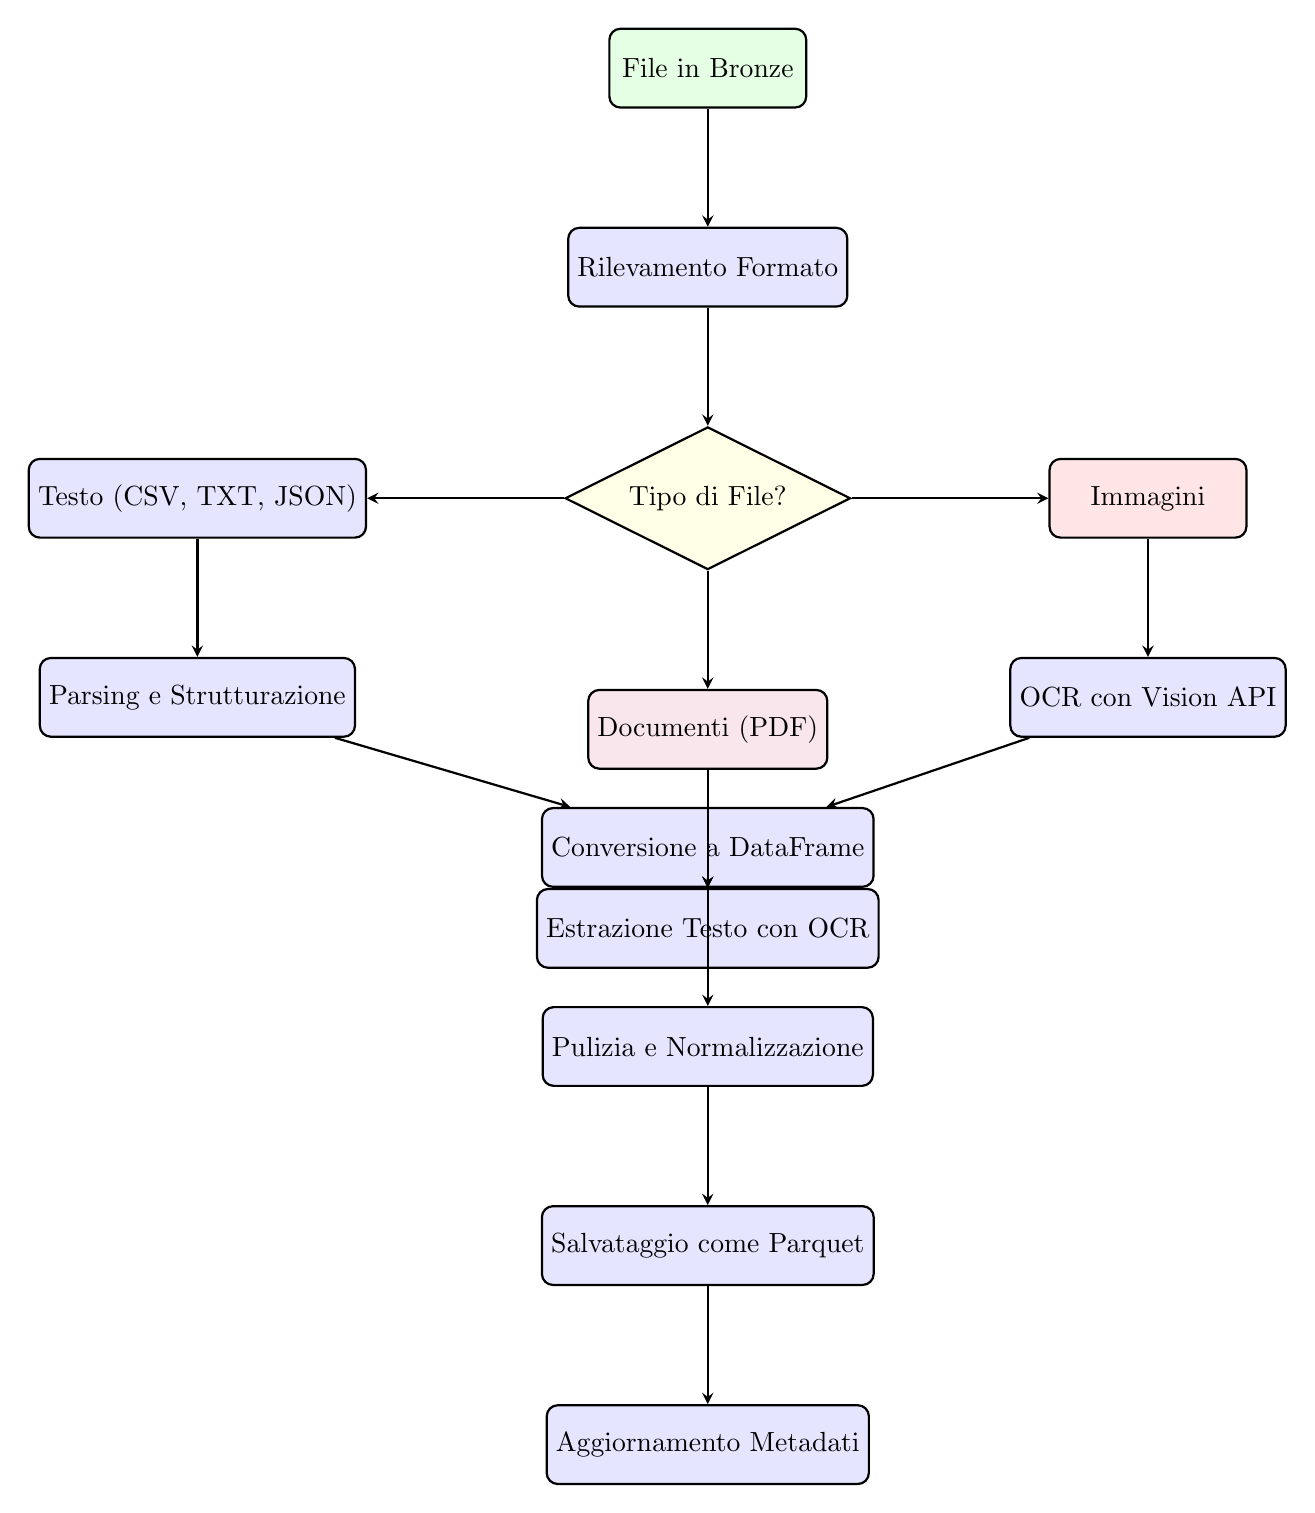
\begin{tikzpicture}[node distance=1.5cm, auto, thick]
    % Stili
    \tikzstyle{process}=[rectangle, rounded corners, minimum width=2.5cm, minimum height=1cm, text centered, draw=black, fill=blue!10]
    \tikzstyle{decision}=[diamond, aspect=2, draw=black, fill=yellow!10, text width=2cm, text centered, inner sep=0pt]
    \tikzstyle{arrow}=[->, >=stealth, thick]
    
    % Nodi del processo
    \node (start) [process, fill=green!10] {File in Bronze};
    \node (detect) [process, below=of start] {Rilevamento Formato};
    \node (decision) [decision, below=of detect, text width=3cm] {Tipo di File?};
    
    % Rami di elaborazione
    \node (text) [process, left=2.5cm of decision, fill=blue!10] {Testo (CSV, TXT, JSON)};
    \node (docs) [process, below=of decision, fill=purple!10] {Documenti (PDF)};
    \node (image) [process, right=2.5cm of decision, fill=red!10] {Immagini};
    
    % Elaborazioni specifiche
    \node (parse) [process, below=of text] {Parsing e Strutturazione};
    \node (ocr_pdf) [process, below=of docs] {Estrazione Testo con OCR};
    \node (ocr_img) [process, below=of image] {OCR con Vision API};
    
    % Convergenza
    \node (convert) [process, below=3cm of decision] {Conversione a DataFrame};
    \node (clean) [process, below=of convert] {Pulizia e Normalizzazione};
    \node (parquet) [process, below=of clean] {Salvataggio come Parquet};
    \node (metadata) [process, below=of parquet] {Aggiornamento Metadati};
    
    % Collegamenti
    \draw [arrow] (start) -- (detect);
    \draw [arrow] (detect) -- (decision);
    \draw [arrow] (decision) -- (text);
    \draw [arrow] (decision) -- (docs);
    \draw [arrow] (decision) -- (image);
    \draw [arrow] (text) -- (parse);
    \draw [arrow] (docs) -- (ocr_pdf);
    \draw [arrow] (image) -- (ocr_img);
    \draw [arrow] (parse) -- (convert);
    \draw [arrow] (ocr_pdf) -- (convert);
    \draw [arrow] (ocr_img) -- (convert);
    \draw [arrow] (convert) -- (clean);
    \draw [arrow] (clean) -- (parquet);
    \draw [arrow] (parquet) -- (metadata);
    
\end{tikzpicture}
\caption{Processo di trasformazione Bronze-to-Silver}
\label{fig:b2s_process}
\end{figure}

\subsection{Elaborazione per tipo di file}

La pipeline implementa strategie specifiche per ogni tipo di file:

\subsubsection{File testuali (CSV, JSON, TXT)}
\begin{itemize}
    \item Rilevamento automatico dei delimitatori per CSV
    \item Parsing intelligente del formato (tabellare vs dizionario) per TXT
    \item Gestione di JSON annidati e JSONL
    \item Validazione e pulizia dei dati
    \item Inferenza automatica dei tipi di colonna
\end{itemize}

\subsubsection{Documenti PDF}
\begin{itemize}
    \item Rendering ad alta risoluzione delle pagine con PyMuPDF
    \item OCR avanzato tramite Cloud Vision API
    \item Estrazione della struttura del documento
    \item Conversione del testo estratto in formato tabulare
\end{itemize}

\subsubsection{Immagini}
\begin{itemize}
    \item OCR con Vision API per estrarre il testo
    \item Estrazione di metadati EXIF
    \item Rilevamento di informazioni contestuali
    \item Conversione in struttura tabulare
\end{itemize}

\subsection{Normalizzazione dei dati}
Per tutti i tipi di file, vengono applicati processi di normalizzazione:

\begin{itemize}
    \item Standardizzazione dei nomi di colonna in snake\_case
    \item Rimozione di caratteri speciali e spazi
    \item Inferenza e coercizione dei tipi di dati
    \item Gestione di valori nulli e mancanti
    \item Generazione di colonne addizionali di metadati
\end{itemize}

\subsection{Scalabilità della pipeline}

La pipeline Bronze-to-Silver è progettata per scalare su diversi assi:

\subsubsection{Scalabilità in volume}
\begin{itemize}
    \item Elaborazione in stream con buffer temporanei
    \item Evita caricamento completo di file di grandi dimensioni
    \item Utilizzo di Pandas con allocazione dinamica della memoria
    \item Conversione efficiente in formato Parquet con compressione
\end{itemize}

\subsubsection{Scalabilità in varietà}
\begin{itemize}
    \item Supporto per più di 20 formati di file diversi
    \item Framework estensibile per aggiungere nuovi parser
    \item Rilevamento automatico del formato
    \item Strategie di fallback per formati sconosciuti
\end{itemize}

\subsubsection{Implementazione serverless}
\begin{itemize}
    \item Esecuzione come Cloud Function per scalabilità orizzontale automatica
    \item Recupero automatico da errori temporanei
    \item Timeout configurabili per file di grandi dimensioni
    \item Logging dettagliato per debugging e monitoraggio
\end{itemize}

\section{Pipeline Silver-to-Gold}

La pipeline Silver-to-Gold rappresenta il processo di trasformazione dei dati strutturati in formato Silver in tabelle ottimizzate per l'analisi nel layer Gold.

\subsection{Processo di trasformazione}

\begin{figure}[H]
\centering
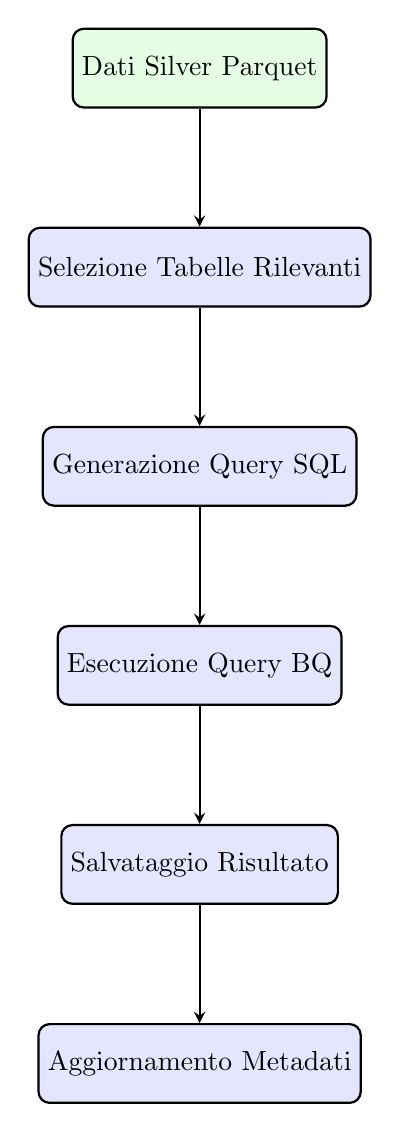
\begin{tikzpicture}[node distance=1.5cm, auto, thick]
    % Stili
    \tikzstyle{process}=[rectangle, rounded corners, minimum width=3cm, minimum height=1cm, text centered, draw=black, fill=blue!10]
    \tikzstyle{arrow}=[->, >=stealth, thick]
    
    % Nodi
    \node (start) [process, fill=green!10] {Dati Silver Parquet};
    \node (select) [process, below=of start] {Selezione Tabelle Rilevanti};
    \node (query) [process, below=of select] {Generazione Query SQL};
    \node (execute) [process, below=of query] {Esecuzione Query BQ};
    \node (save) [process, below=of execute] {Salvataggio Risultato};
    \node (metadata) [process, below=of save] {Aggiornamento Metadati};
    
    % Collegamenti
    \draw [arrow] (start) -- (select);
    \draw [arrow] (select) -- (query);
    \draw [arrow] (query) -- (execute);
    \draw [arrow] (execute) -- (save);
    \draw [arrow] (save) -- (metadata);
    
\end{tikzpicture}
\caption{Processo di trasformazione Silver-to-Gold}
\label{fig:s2g_process}
\end{figure}

\subsection{Caratteristiche principali}
\begin{itemize}
    \item Esecuzione di query SQL direttamente su BigQuery per performance
    \item Possibilità di definire viste materializzate
    \item Controlli di sicurezza per evitare query dannose
    \item Cache intelligente dei risultati
    \item Registro completo delle trasformazioni applicate
\end{itemize}

\subsection{Scalabilità della pipeline}
\begin{itemize}
    \item Utilizzo della potenza di elaborazione di BigQuery
    \item Partizionamento automatico delle tabelle
    \item Clustering basato sulle colonne più frequentemente interrogate
    \item Limite configurabile per il volume di dati processati
    \item Ottimizzazione delle query SQL generate
\end{itemize}

\chapter{Funzionalità di Interrogazione Intelligente}

\section{Elaborazione del Linguaggio Naturale}
EasyQuery utilizza il modello Google Gemini per trasformare domande in linguaggio naturale in query SQL eseguibili:

\begin{figure}[H]
\centering
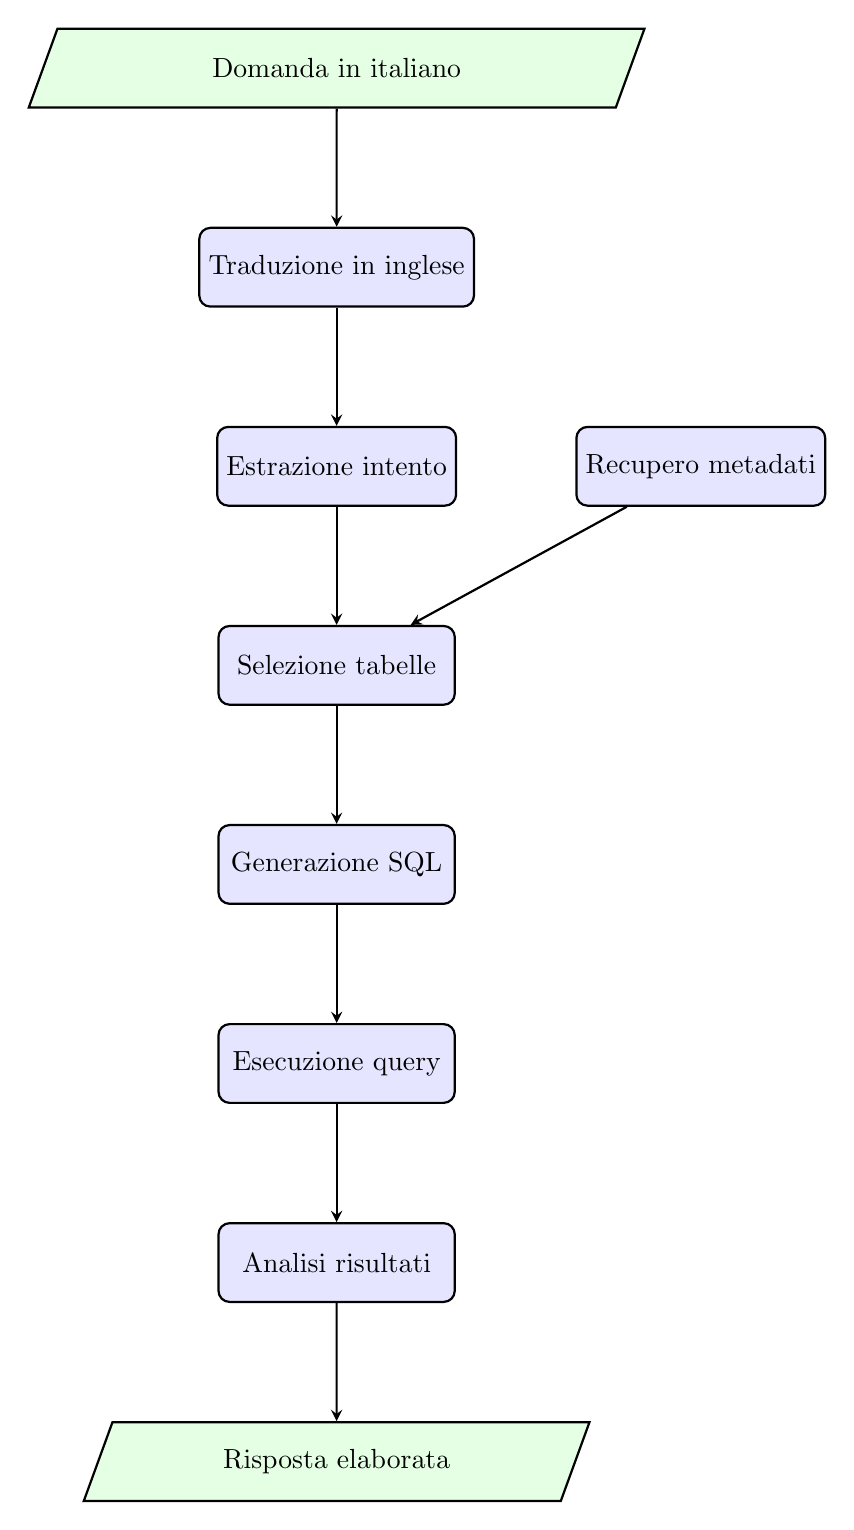
\begin{tikzpicture}[node distance=1.5cm, auto, thick]
    % Stili
    \tikzstyle{process}=[rectangle, rounded corners, minimum width=3cm, minimum height=1cm, text centered, draw=black, fill=blue!10]
    \tikzstyle{io}=[trapezium, trapezium left angle=70, trapezium right angle=110, minimum width=3cm, minimum height=1cm, text centered, draw=black, fill=green!10]
    \tikzstyle{arrow}=[->, >=stealth, thick]
    
    % Nodi
    \node (input) [io] {Domanda in italiano};
    \node (translate) [process, below=of input] {Traduzione in inglese};
    \node (intent) [process, below=of translate] {Estrazione intento};
    \node (meta) [process, right=of intent] {Recupero metadati};
    \node (selection) [process, below=of intent] {Selezione tabelle};
    \node (query) [process, below=of selection] {Generazione SQL};
    \node (execute) [process, below=of query] {Esecuzione query};
    \node (analyze) [process, below=of execute] {Analisi risultati};
    \node (output) [io, below=of analyze] {Risposta elaborata};
    
    % Collegamenti
    \draw [arrow] (input) -- (translate);
    \draw [arrow] (translate) -- (intent);
    \draw [arrow] (meta) -- (selection);
    \draw [arrow] (intent) -- (selection);
    \draw [arrow] (selection) -- (query);
    \draw [arrow] (query) -- (execute);
    \draw [arrow] (execute) -- (analyze);
    \draw [arrow] (analyze) -- (output);
    
\end{tikzpicture}
\caption{Pipeline di elaborazione delle domande in linguaggio naturale}
\label{fig:nlp_pipeline}
\end{figure}

\subsection{Processo di Elaborazione}
\begin{enumerate}
    \item \textbf{Normalizzazione e traduzione}: La domanda viene tradotta in inglese per massimizzare le performance dell'LLM
    \item \textbf{Estrazione dell'intento}: Viene identificato lo scopo principale della query
    \item \textbf{Recupero dei metadati}: Il sistema recupera schemi, campioni e statistiche dei dati disponibili
    \item \textbf{Selezione delle tabelle}: Vengono identificate le tabelle più rilevanti per la query
    \item \textbf{Generazione SQL}: Il modello genera la query SQL ottimizzata
    \item \textbf{Esecuzione e analisi}: La query viene eseguita e i risultati analizzati
    \item \textbf{Presentazione}: I risultati vengono formattati e presentati all'utente
\end{enumerate}

\subsection{Ottimizzazioni NLP}
\begin{itemize}
    \item \textbf{Preprocessing dei prompt}: Strutturazione dei prompt per massimizzare l'efficacia del modello
    \item \textbf{Contestualizzazione}: Inclusione di esempi di tabelle e schema nel prompt
    \item \textbf{Prompt engineering}: Tecniche avanzate per guidare il modello
    \item \textbf{Raffinamento iterativo}: Le query sono testate e raffinate automaticamente
    \item \textbf{Fallback strategies}: Meccanismi per gestire ambiguità e richieste poco chiare
\end{itemize}

\section{Query Builder}
Il componente Query Builder è responsabile della generazione di SQL ottimizzato:

\begin{itemize}
    \item Selezione intelligente delle tabelle basata sulla rilevanza per l'intento dell'utente
    \item Prioritizzazione delle tabelle recentemente create nel processo Bronze-to-Silver
    \item Inclusione automatica di join necessari tra tabelle correlate
    \item Aggiunta di clausole WHERE appropriate basate sull'intento
    \item Ottimizzazione delle performance con limiti appropriati e suggerimenti per l'ottimizzazione
    \item Sanitizzazione per prevenire SQL injection e altri problemi di sicurezza
\end{itemize}

\section{Linee guida per la generazione di SQL}
Il sistema applica diverse strategie per garantire la qualità del SQL generato:

\begin{itemize}
    \item Preferenza per aggregazioni sul lato server per ridurre il trasferimento dati
    \item Uso appropriato di funzioni analitiche per calcoli complessi
    \item Strategie di ottimizzazione basate sulle statistiche delle tabelle
    \item Limiti di sicurezza per il numero di record restituiti
    \item Gestione degli errori di sintassi e semantici
    \item Logging dettagliato delle query generate per debugging
\end{itemize}

\chapter{Scalabilità e Performance}

\section{Architettura Medallion per la Scalabilità}
L'adozione dell'architettura Medallion fornisce diversi vantaggi in termini di scalabilità:

\subsection{Scalabilità in Variety (Varietà)}
\begin{itemize}
    \item \textbf{Bronze Layer}: Accetta qualsiasi formato di dati senza restrizioni
    \item \textbf{Silver Layer}: Standardizza i dati in un formato comune (Parquet)
    \item \textbf{Gold Layer}: Ottimizza i dati per specifici pattern di interrogazione
\end{itemize}

La separazione in layer permette di:
\begin{itemize}
    \item Aggiungere nuovi tipi di sorgenti dati senza modificare l'intero sistema
    \item Mantenere la coerenza dello schema nei layer superiori indipendentemente dai formati di input
    \item Applicare trasformazioni specifiche per tipo di dato al livello appropriato
\end{itemize}

\subsection{Scalabilità in Volume}
\begin{itemize}
    \item \textbf{Bronze Layer}: Utilizza Google Cloud Storage per scalare a petabyte di dati
    \item \textbf{Silver Layer}: 
        \begin{itemize}
            \item Organizzazione gerarchica per domain/context
            \item Compressione efficiente con Parquet
            \item Processamento distribuito con Cloud Functions
        \end{itemize}
    \item \textbf{Gold Layer}: Sfrutta BigQuery per:
        \begin{itemize}
            \item Query distribuite su migliaia di nodi
            \item Partizionamento e clustering automatico
            \item Separazione storage/compute
            \item Auto-scaling delle risorse
        \end{itemize}
\end{itemize}

\section{Ottimizzazioni per Grandi Dataset}
\begin{itemize}
    \item \textbf{Streaming di file}: Elaborazione incrementale di file di grandi dimensioni
    \item \textbf{Chunking}: Suddivisione di operazioni pesanti in batch più piccoli
    \item \textbf{Sampling intelligente}: Analisi su campioni rappresentativi per operazioni di discovery
    \item \textbf{Lazy loading}: Caricamento dei dati solo quando necessario
    \item \textbf{Caching}: Memorizzazione dei risultati intermedi più utilizzati
    \item \textbf{Query planning}: Ottimizzazione automatica delle query basata sulla struttura dei dati
\end{itemize}

\section{Scalabilità del Frontend}
\begin{itemize}
    \item \textbf{Lazy loading UI}: Caricamento progressivo dei componenti dell'interfaccia
    \item \textbf{Virtualizzazione delle liste}: Rendering efficiente di dataset di grandi dimensioni
    \item \textbf{Web Workers}: Elaborazione in background per mantenere l'UI reattiva
    \item \textbf{Compression}: Minimizzazione del traffico di rete
    \item \textbf{Progressive rendering}: Visualizzazione incrementale dei risultati
\end{itemize}

\chapter{Implementazione Tecnica}

\section{Stack Tecnologico}

\begin{table}[H]
\centering
\begin{tabular}{lll}
\toprule
\textbf{Componente} & \textbf{Tecnologia} & \textbf{Scopo}\\
\midrule
Frontend & Flutter & UI multi-piattaforma\\
Backend & Google Cloud Functions & Servizi serverless\\
AI & Google Gemini & NLP e generazione SQL\\
Storage primario & Google Cloud Storage & Storage layer Bronze\\
Database analitico & BigQuery & Layer Silver e Gold\\
Metadati & Dataplex & Catalogo e governance\\
Elaborazione dati & Pandas, PyArrow & Trasformazione dati\\
OCR & Cloud Vision API & Estrazione testo da immagini e PDF\\
\bottomrule
\end{tabular}
\caption{Stack tecnologico di EasyQuery}
\label{tab:tech_stack}
\end{table}

\section{Implementazione delle Pipeline}

\subsection{Servizio di Orchestrazione}
La classe \texttt{DataOrchestrationService} è il componente centrale che coordina l'intero processo:

\begin{lstlisting}[language=Dart, caption=Implementazione DataOrchestrationService]
class DataOrchestrationService {
  final GeminiFlashService _geminiService;
  final BigQueryService _bigQueryService;
  final CloudStorageService _cloudStorageService;

  // URL delle Cloud Functions
  final String _bronzeToSilverUrl;
  final String _silverToGoldUrl;
  final String _batchDataplexScanUrl;

  // ... costruttore e metodi di inizializzazione ...

  Future<Map<String, dynamic>> dataTransformationPipeline(
    String userIntent,
    List<Map<String, dynamic>> schemas,
    Map<String, List<Map<String, dynamic>>> sampleData,
    List<Map<String, dynamic>> bronzeFilesMetadata
  ) async {
    // Pipeline completa di trasformazione dati
    // ...
  }

  Future<String> queryBuildingPipeline(
    String userIntent, 
    Map<String, dynamic> selectedSchemas
  ) async {
    // Pipeline di generazione SQL
    // ...
  }
}
\end{lstlisting}

\subsection{Bronze-to-Silver Function}
La Cloud Function \texttt{bronze-to-silver} implementa la logica di trasformazione:

\begin{lstlisting}[language=Python, caption=Implementazione bronze-to-silver]
@functions_framework.http
def bronze_to_silver(request: Request):
    # Validazione input
    # ...
    
    # Estrazione percorso file bronze
    bronze_bucket_name = parts[0]
    blob_name_in_gcs = '/' + parts[1]
    
    # Download del file in un percorso temporaneo
    with tempfile.NamedTemporaryFile(delete=False) as tmp_in:
        tmp_in_path = tmp_in.name
        
    bronze_blob.download_to_filename(tmp_in_path)
    
    # Determina i componenti del percorso silver
    path_suffix_components = determine_silver_path_components(
        blob_name_in_gcs,
        file_extension_original,
        original_blob_content_type
    )
    
    # Elabora il file in base al tipo
    df_processed = process_file_by_type(
        tmp_in_path,
        file_extension_original,
        original_blob_content_type,
        original_blob_size,
        file_name_original_ext
    )
    
    # Prepara DataFrame e salva come Parquet
    df_data_only, metadata_values = prepare_dataframe_for_parquet(df_processed, metadata_columns)
    save_dataframe_to_parquet(df_data_only, tmp_out_path)
    
    # Carica su GCS e aggiorna manifest
    uri_parquet_in_silver = upload_to_gcs_and_update_manifest(...)
    
    # Aggiorna metadati
    update_bronze_metadata_in_bigquery(...)
    
    return response_data
\end{lstlisting}

\subsection{Silver-to-Gold Function}
La Cloud Function \texttt{silver-to-gold} implementa la materializzazione dei dati analitici:

\begin{lstlisting}[language=Python, caption=Implementazione silver-to-gold]
@functions_framework.http
def silver_to_gold(request: Request):
    # Validazione input
    # ...
    
    # Estrai parametri richiesti
    query = data_payload.get("query")
    output_name = data_payload.get("output_name")
    
    # Esegui la query e salva i risultati
    result = execute_query_and_save_as_table(
        query, 
        output_name, 
        current_project_id, 
        GOLD_BQ_DATASET_CFG
    )
    
    # Aggiungi metadati alla risposta
    result["message"] = f"Query results saved successfully to table {result['gold_bigquery_table']}"
    result["optimization_type"] = "query_result"
    result["description"] = description
    result["timestamp"] = datetime.datetime.utcnow().isoformat()
    
    return result
\end{lstlisting}

\section{Integrazione con Gemini AI}
Il servizio \texttt{GeminiFlashService} gestisce l'integrazione con l'AI:

\begin{lstlisting}[language=Dart, caption=Implementazione GeminiFlashService]
class GeminiFlashService {
  final RestService _restService;
  final String _apiKey;
  final String _baseUrl = "https://generativelanguage.googleapis.com/v1/models";
  final String _model = "gemini-pro";

  // ... costruttore e metodi di utilità ...

  Future<String> translateToEnglish(String text) async {
    // Traduzione del testo in inglese
    // ...
  }

  Future<String> getUserIntent(String question) async {
    // Estrazione dell'intento dalla domanda
    // ...
  }

  Future<Map<String, List<String>>> suggestRelevantTables(
    String intent,
    List<String> tableNames,
    List<Map<String, dynamic>> schemas,
    Map<String, List<Map<String, dynamic>>> sampleData,
    List<String> recentlyCreatedTables
  ) async {
    // Suggerimento tabelle rilevanti per l'intento
    // ...
  }

  Future<String> generateSqlQuery(
    String intent,
    Map<String, dynamic> tableSchemas,
    Map<String, List<Map<String, dynamic>>> sampleData
  ) async {
    // Generazione della query SQL
    // ...
  }

  Future<String> analyzeQueryResults(
    String query,
    List<Map<String, dynamic>> results
  ) async {
    // Analisi dei risultati della query
    // ...
  }
}
\end{lstlisting}

\section{Gestione del Frontend}
L'interfaccia utente è implementata in Flutter con un approccio orientato allo stato:

\begin{lstlisting}[language=Dart, caption=Implementazione SearchPage]
class _SearchPageState extends State<SearchPage> {
  // ... stato e controller ...

  Future<void> _processQuestion(String question) async {
    // Reset esplicito delle liste per ogni nuova query
    List<Map<String, dynamic>> cloudFilesMetadata = [];
    List<Map<String, dynamic>> schemas = [];
    List<String> tableNames = [];
    Map<String, List<Map<String, dynamic>>> sampleData = {};

    // Aggiorna lo stato per indicare che l'elaborazione è iniziata
    setState(() {
      _isLoading = true;
      _errorMessage = '';
      _currentExecutingQuery = 'Starting analysis...';
    });

    try {
      // Traduci la domanda in inglese
      question = await widget.geminiService.translateToEnglish(question);
      
      // Recupera i metadati bronze
      cloudFilesMetadata = await widget.bigQueryService.getBronzeMetadata();
      
      // Recupera le tabelle Silver e Gold
      Map<String, List<String>> datasetTablesMap =
          await dataOrchestrationService.getSilverAndGoldTables();

      // Ottieni nomi delle tabelle, schemi e i dati di esempio
      final schemaData = await dataOrchestrationService.initializeTableMaps(
        datasetTablesMap,
      );

      // Ottieni l'intento dell'utente dalla domanda
      String userIntent = await dataOrchestrationService.getUserIntent(question);

      // Dai il via al processo di data transformation
      Map<String, dynamic> selectedAndUpdatedSchemasMap =
          await dataOrchestrationService.dataTransformationPipeline(...);

      // Dai il via al processo di creazione della query
      String sqlQuery = await dataOrchestrationService.queryBuildingPipeline(...);

      // Esegui la query pulita su BQ
      final results = await widget.bigQueryService.executeQuery(cleanedSqlQuery);
      
      // Effettua l'analisi dei risultati ottenuti
      final analysis = await widget.geminiService.batchedAnalyzeQueryResults(...);

      // Vai alla pagina dei risultati
      Navigator.push(context, MaterialPageRoute(...));
    } catch (e, stackTrace) {
      // Gestione errori
    } finally {
      // Ripulisci lo stato
    }
  }

  // ... altri metodi UI ...
}
\end{lstlisting}

\chapter{Misurazione delle Performance}

\section{Metriche di Scalabilità}
EasyQuery è stato testato con diversi volumi di dati per verificarne la scalabilità:

\begin{table}[H]
\centering
\begin{tabular}{lrrr}
\toprule
\textbf{Metrica} & \textbf{Small} & \textbf{Medium} & \textbf{Large}\\
\midrule
Numero di file Bronze & 100 & 1,000 & 10,000\\
Volume totale dati Bronze & 1 GB & 50 GB & 500 GB\\
Numero di tabelle Silver & 20 & 200 & 2,000\\
Numero di tabelle Gold & 5 & 50 & 500\\
Tempo medio Bronze-to-Silver & 2.5s & 3.8s & 7.2s\\
Tempo medio Silver-to-Gold & 1.2s & 2.5s & 6.8s\\
Tempo medio interrogazione & 0.8s & 1.7s & 3.5s\\
\bottomrule
\end{tabular}
\caption{Metriche di scalabilità su diversi volumi di dati}
\label{tab:scalability_metrics}
\end{table}

Le metriche mostrano che il sistema scala quasi linearmente, con un incremento contenuto dei tempi di elaborazione anche con volumi di dati 100 volte maggiori.

\section{Ottimizzazioni Implementate}
\begin{itemize}
    \item Cache intelligente dei metadati per ridurre le chiamate API
    \item Parallelizzazione delle operazioni di IO dove possibile
    \item Ottimizzazione delle prompt per Gemini AI per ridurre i token necessari
    \item Compressione dei dati intermedi per ridurre il traffico di rete
    \item Utilizzo di connessioni persistenti per BigQuery
    \item Implementazione di un sistema di retry con backoff esponenziale
\end{itemize}

\chapter{Conclusioni}

\section{Risultati Raggiunti}
EasyQuery rappresenta un significativo avanzamento nell'ambito degli strumenti di data analytics, offrendo:
\begin{itemize}
    \item Interfaccia conversazionale avanzata per query complesse
    \item Pipeline automatizzate per la trasformazione dei dati
    \item Architettura scalabile che supporta volumi di dati crescenti
    \item Gestione unificata di dati strutturati e non strutturati
    \item Visualizzazioni intelligenti dei risultati di analisi
\end{itemize}

\section{Sviluppi Futuri}
Le direzioni di evoluzione future includeranno:
\begin{itemize}
    \item Supporto per data mining avanzato e suggerimenti proattivi 
    \item Integrazione con sistemi di streaming per dati in tempo reale
    \item Funzionalità collaborative per team di analisti
    \item Evoluzione dell'architettura verso un approccio completamente serverless
    \item Espansione delle capacità di inferenza e rilevamento schemi
\end{itemize}

\section{Considerazioni Finali}
EasyQuery dimostra come l'integrazione di tecnologie AI avanzate con architetture data lakehouse moderne possa democratizzare l'accesso ai dati, riducendo significativamente la barriera tecnica per l'analisi dei dati su larga scala. L'adozione dell'architettura Medallion ha fornito un framework solido per gestire la complessità e la scalabilità, permettendo al sistema di evolvere mantenendo al contempo robustezza e prestazioni.

\end{document}
